\documentclass[
% Options for apa7
    a4paper,                % Paper size
    11pt,                   % Font size
    stu,                    % Format as assignment
    % donotrepeattitle,       % Start body text without repeating title
    floatsintext,           % Insert tables and figures with texts
    biblatex,               % Use BibLaTeX for references
% Options for hyperref
    colorlinks=true,        % Colour all links
    linkcolor=red,          % Cross-references in red
    anchorcolor=black,      % Keep anchors black
    citecolor=blue,         % In-text-referencs in blue
    urlcolor=blue,          % DOIs and URLs are in blue
    bookmarks=true,         % Generate bookmarks for PDF readers
    bookmarksopen=false,    % Expand all bookmarks as default
    bookmarksnumbered=true, % Keep section number in bookmarks
    % Options for xcolor
    dvipsnames              % Use colour BrickRed and PineGreen
]{apa7}

% Specify absolute path to the tt.sty file, depending on the operating system
\usepackage{ifplatform}
\ifwindows
    \usepackage{M:/pc/Dokumenter/tt}
\fi
\iflinux
    \usepackage{/home/tony/uio/pc/Dokumenter/tt} % Must not use ~ for home directory. Spell in full.
\fi
\ifmacosx
    \usepackage{/Users/tctan/uio/pc/Dokumenter/tt}
\fi

% Specify relative path to Master bib file
\addbibresource{../Bibliography/Master.bib}

\title{Identifying Inter-subject Difficulties in Norwegian GPA Data}
\authorsnames{Tony C. A. Tan}
\authorsaffiliations{{Centre for Educational Measurement, University of Oslo}}
\course{Continuous Draft}
\professor{Prof Rolf V. Olsen \& Dr Astrid M. J. Sands{\o}r}
\duedate{V{\aa}r 2023}

% \abstract{
[Follow publisher's instructions.]

% Fairness is both an essential and an elusive integral of educational assessment. Following \poscite{gipps:2009} social-cultural framing of assessment fairness and \poscite{tierney:2017} democratic--measurement--pedagogical construction, the current study models GPA as a selection device \parencite{kane:2013} for accessing privileged social resources \parencite{bourdieu:1973}. It addresses the construct validity of GPAs by examining any construct-irrelevant variance \parencite{messick:1989} related to students' subject choices.

% %\subsection{Methodology}

% Item response theory is particularly suitable for extracting item difficulty information in order to study assessment's selection fairness. This study considers each GPA subject as an item and each candidate as a person. Using marginal maximum likelihood (MML) estimation, the analyses will ascertain difficulty parameters for all major subjects in Norwegian upper secondary schools. Registry data containing Norwegian students' GPA performance in 2019 are first regularised by removing subjects with fewer than 1,000 candidates and by only including candidates who have received valid GPAs through upper secondary school completions. Next, subject difficulty parameters will be extracted using generalised partial credit models \parencite[GPCM,][]{muraki:1992}. Lastly, group invariance tests are applied to assess the extent to which selection bias had impacted on subject difficulty parameter estimates.

% %\subsection{Expected Results}

% The registry data set will be available for analysis in short time and the described analyses will be presented and discussed at the conference. We expect Norway's GPA subjects to differ in difficulties \parencite{he:2018} and to exhibit significant selection effects \parencite{korobko:2008}.

% %\subsection{Relevance to Nordic Educational Research}

% Given that university entries in Europe is largely based on the final grades from secondary schooling, the presented analysis is likely to be relevant to other countries using grades as the selection criteria into tertiary education. The issue of potential unequal treatment of students with different specialisation in upper secondary school applies beyond the Norwegian context. By testing the assumption that grades from different specialities support GPA's selection purpose equally well, this study lends statistical support to evidence-based policy formation process commonly practised in the Nordic community and serves to strengthen the fairness of our merit-based university admission decisions.
}

\keywords{grade point average, Norway, item response theory, assessment fairness, group invariance}


\begin{document}
\maketitle

% %\section{Introduction} % Do not include the word "Introduction" as a Level 1 heading. Just start intro as a normal paragraph immediately after the title.
  % Use \input{} for Intro.tex so that the title and the first paragraph stay on the same page.

\section{Conceptual Framework}


\subsection{Missing Data Treatment}

IRT item parameter estimations demand strong assumptions on the data missing mechanism. Joint, conditional and marginal maximum likelihood procedures are only valid under ``ignorable non-response'' conditions where missing propensities are related to neither item nor person parameters \parencite{molenaar:1995}. When test takers skip items after seeing their content, for example, the ignorablity condition is unlikely to hold \parencite{mislevy:1987}, neither are tests with items not reached due to time constraint \parencite{lord:1974, lord:1983}. In the current study involving Norway's GPA archive, missing records are not the result of randomly assigning candidates to subjects (not MCAR), nor are each candidate's missing GPAs independent of observed ones (not MAR). In fact, missing patterns are likely to be related to both personal capabilities and subject difficulties with low ability candidates self-selecting into easy subjects while difficult subjects attracting only high capability students. Resultantly, MML estimates of subject difficulties after marginalising personal parameters are no longer unbiased \parencite[][Table 2]{mislevy:1988}.

Literature has congregated into three main approaches for the purpose of addressing missing values. In the \emph{classical approaches}, missing responses can be (a) ignored and treated as non-administered, (b) coded as incorrect, or (c) assigned fractional correct values. This procedure is widely practised amongst international large-scale assessment analysts \parencite{pohl:2014}. Secondly, \emph{imputation-based approaches} encompass corrected mean substitution, response function imputation, EM algorithm and multiple imputation (MI). \textcite{finch:2008} compared the performance of competing imputation-based methods and found MI to be the optimal procedure. MI considers (a) candidates' valid responses, (b) the responses of similar participants, and (c) observed information on covariates if a background model is available, in imputing the missing responses. This Bayesian approach generates multiple draws from parameters' posterior distributions to form correct standard errors \parencite{carpenter:2013}. MI also reallocates the missing-data burden from the analysis stage to the data preparation stage \parencite{reiter:2007}, therefore re-enabling subsequent inferences whose validity depends on complete-data statistical methods and software \parencite[][Chapter 4]{rubin:1987}. Lastly, the recently developed \emph{model-based approaches} include missing tendency in the IRT model when estimating item and person parameters via either (a) latent missing propensity \parencite{holman:2005, glas:2008, glas:2015,korobko:2008} or (b) manifest approach \parencite{rose:2010}.

Both MI and model-based approaches carry their corresponding costs. Studies interested in person parameters shall employ plausible values as the appropriate strategy \parencite{mislevy:1991,mislevy:1993}. But plausible values themselves are multiple imputations of (already multiple imputed) latent variables, causing a cascade of computation demand in the form of nested MI, limiting its wide use in practice such as large-scale assessments or competence tests \parencite{pohl:2014}. Model-based approaches, on the other hand, may generate biased parameter estimates should the missing propensity violate the unidimensionality assumption \parencite{rose:2013}. The current study focuses on \emph{item} parameters (i.e., subject difficulties) while treating person parameters as ``nuisance'' by integrating it out of the maximum likelihood, thereby avoids the MI cascade problem. The risk of committing unidimensionality violation at the missing propensity estimation stage, however, is material since it is not implausible to expect more than one behavioural patterns in young students' GPA choice decisions. It is based on these cost-benefit considerations that this project prefers the MI-based approach to missing data over the model-based procedure.

\section{Methods}

\subsection{Population}

This study retains the entire cohort of Norway's Year 10 students graduating in 2019 as its targeted population. Students' GPA (\textit{grunnskolepoeng}), teacher-assigned grades (\textit{standpunktkarakter}), as well as written (\textit{SKR}) and oral (\textit{MUN}) exam grades were extracted from the national register. This data source is unique because it is the \emph{population}, rather than samples, that forms our unit of analysis. Academic attainment records were then re-shaped into the format that each candidate occupies one row and each subject is represented by one column. This process led to a preliminary data set of 64,918 students and 200 subjects. Next, $4,300$ students without valid GPA records were excluded from subsequent analyses, representing a loss rate of $6.62\%$. Seventeen subjects were retained based on these inclusion criteria:

\subsubsection{Teacher-assigned Grades (12 subjects)}

Under the Norwegian education system, Year 10 students shall complete 13 compulsory subjects as well as electives. This study included all compulsory subjects except for Sidem{\aa}l.\footnote{The Norwegian language has two official written forms: Bokm{\aa}l and Nynorsk, with the former being more prevalent in the media. Students growing up in one written form must enroll the other as their Sidem{\aa}l, unless Norwegian is not their native language. Nynorsk users tend to have easier time in Sidem{\aa}l due to existing exposure to Bokm{\aa}l. Bokm{\aa}l users, on the other hand, find Nynorsk more challenging while fulfilling Sidem{\aa}l. Since Sidem{\aa}l contains two sub-cohorts with distinct difficulty profiles, we opt not to include this subject in our analyses.} We applied equal treatment to courses instructed in Norwegian and in Sami language by merging these records.\footnote{For example, \href{https://www.udir.no/kl06/nat0010}{NAT0010 Naturfag 10. {\aa}rstrinn} and \href{https://www.udir.no/kl06/nat0020}{NAT0020 Naturfag, samisk plan, 10. {\aa}rstrinn} were merged into one subject Natural Sciences. If academic results were available from both instruction languages, we retained the higher grades during merging.} Twelve teacher-assigned grades were included for our analysis: Written Norwegian (NORW), Oral Norwegian (NORO), Written English (ENGW), Oral English (ENGO), Mathematics (MATH), Natural Sciences (NATS), Social Sciences (SOCS), Religion (RELI), Music (MUSI), Arts and Handcraft (HAND), Food and Health (FOOD), and Physical Education (PHED).

\subsubsection{Written Exam Grades (3 subjects)}

Norway uses a lottery draw to randomly assign Year 10 students to participate in \emph{one} of the following three written exams: Norwegian (E-NORW), English (E-ENGW) and mathematics (E-MATH). This ``planned missingness'' implies that although numeral in quantity, the unobserved exam grades can be safely modelled under the missing completely at random (MCAR) assumption \parencite{little:2019}.\footnote{Even if the lottery is less than perfectly random, Rasch models are still valid under the weaker assumption of missing at random (MAR), as long as one is satisfied that missing propensities are unrelated to item or person parameters \parencite{molenaar:1995}.} Rasch models have a major advantage for handling missing values thanks to the sufficient overlap across subjects in the score matrix \parencite{he:2018}.

\subsubsection{Oral Exam Grades (2 subjects)}

Year 10's oral exams consist of the same three subjects as in written exams, plus a wide selection such as natural and social sciences, with students being randomly assigned into \emph{one} oral exam by lottery. In order to better match teacher-assigned grades, only Oral Norwegian (E-NORO) and Oral English (E-ENGO) were included in this study. Since students are spread thinly across many oral exam subjects, E-NORO and E-ENGO appeared more sparse than their teacher-assigned counterparts, leading to larger confidence intervals in subsequent analyses.


\section{Results}

\subsection{Descriptive Statistics}

\cref{tab:descriptive} summarised key information about the 18 \textsc{gpa} subjects examined by this study, including the number of valid entries, grade distributions, and links to official documentation. It is firstly noticeable that data missing rates differed significantly across modes of assessment. Teacher-assigned grades carried small missing percentages most under 5 percent, hence imposing little concerns over estimation bias. Although written- and oral-exams had large missing percentages, this was the effect of the equal-probability sampling procedures. Under planned missingness, the observed grades represent unbiased estimates of true grades despite only 1/3 or 1/5 of the students were studied.

Secondly, grade distributions differed both between- and within-modes of assessment. A large number of grade counts clustered around Grade 3 and 4 for external exams, whereas teacher-assigned grades peaked at different bands depending on the subject, with \textsc{math} mainly covering Grade 2 to 4 while \textsc{food} covering largely Grade 4 and 5.

\subsection{Subject Difficulties}

\subsubsection{Overall Difficulties}
\textsc{gpa} subjects' overall difficulties are shown in \cref{fig:expected}. Using \textsc{math} as an example, the horizontal axis of Panel A represents students' latent competencies, ranging from low ($\theta=-10$) to high ($\theta=5$), and the vertical axis represents grades randing from $1$ to $6$. Students with low competencies are expected to receive Grade 1 while Grade 6 is reserved to students with very high competencies. Mapping every competency level to its expected grade yields the sigmoid curve in Panel A. Furthermore, there exists a median student, who evenly divides \textsc{math}'s observations into 50\% below, and 50\% above him/her, whose $\theta$ is defined as zero. Tracing this median student's expected score from the curve in Panel A, one reads a grade of 3.64 as the \emph{overall difficulty} for \textsc{math}. Repeating this procedure for all 18 GPA subjects gave rise to the scatter plot in Panel B. Subject with low expected grades such as \textsc{math} are more difficult while \textsc{phed} and \textsc{food} are easy subjects evidenced by the high expected grades from median students.

Ranked by overall difficulties, teacher-assigned grades appeared to align themselves along the \textit{manu}--\textit{mente} dichotomy. A median student is expected to receive a score one grade lower in the most difficult subject \textsc{math} than from the easiest one \textsc{phed}. Written exams are more difficult than oral exams, with \textsc{nor\_w} being more difficult than teacher-assigned \textsc{math}. Oral English exam, in contrast, is comparable in difficulty to \textit{mente} subjects such as teacher-assigned \textsc{food}.

\subsubsection{Grade-level Difficulties}
This study operationalises grade-level difficulties using difficulty thresholds. For a polytomous \textsc{irt} item such as \textsc{math}, a category characteristic curve (\textsc{ccc}) describes the likelihood a particular grade is received by students with varying competency levels. The $P1$ curve in Panel A \cref{fig:grade_level}, for example, states that Grade 1 is awarded to students with low competencies almost surely (probability approaching 1) but to those with high competencies almost never (probability approaching 0). Similarly, the $P2$ curve suggests that Grade 2 is most likely to be awarded to students with competencies between approximately $\theta=[-6, -1]$ but low probabilities outside this domain. The intersection between $P1$ and $P2$ marks a difficulty threshold $\delta_1$, above which the next grade is more likely. Six \textsc{ccc}s produce five difficulty thresholds $\delta_1, \dots, \delta_5$, which concisely summarise each subject's \emph{grade-level difficulties}. Repeating this procedure to all 18 \textsc{gpa} subjects produces Panel B.

Among teacher-assigned grades, the competency demands for receiving a particular grade differed widely depending on the low- and high-end of the grading scale. High consistency was observed at the $\delta_5$-level where all subjects required students to have high competencies ($\theta \approx 2.5$) to transitions from Grade 5 to the top grade 6. As one moves down the grade ladder, however, the difficulty gap expanded to more than one grade between the most difficult subject and the easiest one such that a Grade 3 in \textsc{math} is more comparable to a Grade 4 in \textsc{food}. Lastly, the lengthening 95\% confidence intervals in $\delta_1$ suggests that teachers did not fully utilise the entire grade scale, especially for the \textit{manu} subjects---an observation corroborated by the grade distributions in \cref{tab:descriptive}.

\subsection{Model Fit Measures and Information Curves}

\cref{fig:fit} visualises the Rasch model fit statistics using the 2019 Year 10 \textsc{gpa} data. A model with perfect fit would generate an information weighted fit (infit) and unweighted fit mean square (outfit) of $1$ \parencite{wu:2016}. Infit and outfit mean squares below $1$ suggest overfit where the item is more discriminating than the average item discrimination. Resultantly, \textcite{wu:2016} consider high quality items (\textit{mente} subjects) to have mean squares less than $1$ even though some of these items may be deemed as misfitting the model. \textsc{gpa} subjects with mean squares much greater than $1$ are deemed poorer \textsc{irt} items. Under these criteria, teacher-assigned grades for \textit{manu} subjects \textsc{hand}, and \textsc{phed} showed poor model fit, as well as oral English exam grades.

Lastly, \cref{fig:info} presents the information curves (left scale, blue) for the 18 \textsc{gpa} subjects. An information curve plots the information function against the latent competency. The information function is the expected information gained from a student's response to an item given their competency level. \cref{fig:info} also displays the standard error curves (right scale, red) that communicate the precision of each Rasch item over the competency range. The information and standard error curves jointly suggest that the Rasch model used in this study provided strong explanatory power and high precision over the mid-range of the latent competency scale where most students reside.


% \section{Discussions}

What does all this mean? Well, let me make you a cup of tea first.

\printbibliography

\ttltable{tab:descriptive}{Descriptive Statistics for the 18 GPA Subjects}{
    \begin{tabular}{clrrrrrrrrrl}
        \toprule
    Subject & \multicolumn{1}{c}{Subject} & \multicolumn{1}{c}{Valid} & \multicolumn{1}{c}{Missing} & \multicolumn{1}{c}{Missing} & \multicolumn{6}{c}{Grade Frequency}           & \multicolumn{1}{c}{\textsc{udir}} \\
    \cmidrule{6-11}    Code  & \multicolumn{1}{c}{Name} & \multicolumn{1}{c}{Entries} & \multicolumn{1}{c}{($n$)} & \multicolumn{1}{c}{($\%$)} & \multicolumn{1}{c}{1} & \multicolumn{1}{c}{2} & \multicolumn{1}{c}{3} & \multicolumn{1}{c}{4} & \multicolumn{1}{c}{5} & \multicolumn{1}{c}{6} & \multicolumn{1}{c}{Course Code} \\
        \midrule
        \multicolumn{12}{l}{\textbf{Teacher-assigned Grades} (12 subjects)}\\
    \textsc{math}  & Mathematics & 59,184 & 1,434 & 2.37  & 1,165 & 10,086 & 15,447 & 15,443 & 12,520 & 4,523 & \href{https://www.udir.no/lk20/fagkoder/mat0010}{\textsc{mat0010}} \\
    \textsc{norw}  & Written Norwegian & 58,946 & 1,672 & 2.76  & 498   & 5,504 & 15,503 & 20,482 & 13,888 & 3,071 & \href{https://www.udir.no/lk20/fagkoder/nor0214}{\textsc{nor0214}} \& \href{https://www.udir.no/lk20/fagkoder/nor0041}{\textsc{nor0041}} \\
    \textsc{engw}  & Written English & 59,047 & 1,571 & 2.59  & 850   & 5,315 & 13,671 & 19,934 & 14,937 & 4,440 & \href{https://www.udir.no/lk20/fagkoder/eng0012}{\textsc{eng0012}} \\
    \textsc{nats}  & Natural Sciences & 59,642 & 976   & 1.61  & 490   & 4,801 & 12,134 & 17,179 & 17,448 & 7,590 & \href{https://www.udir.no/lk20/fagkoder/nat0010}{\textsc{nat0010}} \& \href{https://www.udir.no/lk20/fagkoder/nat0020}{\textsc{nat0020}} \\
    \textsc{noro}  & Oral Norwegian & 58,982 & 1,636 & 2.70  & 210   & 2,994 & 10,855 & 18,764 & 19,254 & 6,905 & \href{https://www.udir.no/lk20/fagkoder/nor0216}{\textsc{nor0216}} \& \href{https://www.udir.no/lk20/fagkoder/nor0042}{\textsc{nor0042}} \\
    \textsc{engo}  & Oral English & 59,148 & 1,470 & 2.43  & 441   & 3,200 & 9,938 & 19,725 & 18,947 & 6,897 & \href{https://www.udir.no/lk20/fagkoder/eng0013}{\textsc{eng0013}} \\
    \textsc{reli}  & Religion & 56,993 & 3,625 & 5.98  & 316   & 3,386 & 9,928 & 16,966 & 18,293 & 8,104 & \href{https://www.udir.no/lk20/fagkoder/RLE0030}{\textsc{rle0030}} \& \href{https://www.udir.no/lk20/fagkoder/rel0040}{\textsc{rel0040}} \\
    \textsc{socs}  & Social Sciences & 59,715 & 903   & 1.49  & 307   & 3,466 & 10,489 & 17,527 & 19,538 & 8,388 & \href{https://www.udir.no/lk20/fagkoder/saf0010}{\textsc{saf0010}} \& \href{https://www.udir.no/lk20/fagkoder/saf0020}{\textsc{saf0020}} \\
    \textsc{musi}  & Music & 57,716 & 2,902 & 4.79  & 120   & 1,450 & 6,771 & 18,830 & 22,940 & 7,605 & \href{https://www.udir.no/lk20/fagkoder/mus0010}{\textsc{mus0010}} \& \href{https://www.udir.no/lk20/fagkoder/mus0020}{\textsc{mus0020}} \\
    \textsc{hand}  & Arts and Handcraft & 58,001 & 2,617 & 4.32  & 93    & 1,142 & 6,876 & 19,744 & 23,140 & 7,006 & \href{https://www.udir.no/lk20/fagkoder/khv0010}{\textsc{khv0010}} \& \href{https://www.udir.no/lk20/fagkoder/khv0020}{\textsc{khv0020}} \\
    \textsc{phed}  & Physical Education & 57,731 & 2,887 & 4.76  & 102   & 913   & 4,612 & 16,606 & 26,037 & 9,461 & \href{https://www.udir.no/lk20/fagkoder/kro0020}{\textsc{kro0020}} \\
    \textsc{food}  & Food and Health & 57,683 & 2,935 & 4.84  & 16    & 561   & 6,060 & 19,098 & 23,907 & 8,041 & \href{https://www.udir.no/lk20/fagkoder/mhe0010}{\textsc{mhe0010}} \& \href{https://www.udir.no/lk20/fagkoder/mhe0020}{\textsc{mhe0020}} \\
        \multicolumn{12}{l}{\textbf{Written Exam Grades} (3 subjects)}\\
    \textsc{mat\_w} & Written Mathematics & 15,252 & 45,366 & 74.84 & 235   & 2,482 & 4,261 & 4,529 & 2,902 & 843   & \href{https://www.udir.no/lk20/fagkoder/mat0010}{\textsc{mat0010}} \\
    \textsc{nor\_w} & Written Norwegian & 13,851 & 46,767 & 77.15 & 237   & 2,345 & 5,245 & 4,106 & 1,616 & 302   & \href{https://www.udir.no/lk20/fagkoder/nor0214}{\textsc{nor0214}} \\
    \textsc{eng\_w} & Written English & 14,723 & 45,895 & 75.71 & 225   & 1,573 & 4,224 & 4,940 & 2,913 & 848   & \href{https://www.udir.no/lk20/fagkoder/eng0012}{\textsc{eng0012}} \\
        \multicolumn{12}{l}{\textbf{Oral Exam Grades} (3 subjects)}\\
    \textsc{mat\_o} & Oral Mathematics & 8,838 & 51,780 & 85.42 & 16    & 770   & 2,041 & 2,503 & 1,958 & 1,550 & \href{https://www.udir.no/lk20/fagkoder/mat0011}{\textsc{mat0011}} \\
    \textsc{nor\_o} & Oral Norwegian & 9,310 & 51,308 & 84.64 & 34    & 459   & 1,651 & 2,520 & 2,342 & 2,304 & \href{https://www.udir.no/lk20/fagkoder/nor0216}{\textsc{nor0216}} \\
    \textsc{eng\_o} & Oral English & 9,207 & 51,411 & 84.81 & 36    & 330   & 1,405 & 2,651 & 2,452 & 2,333 & \href{https://www.udir.no/lk20/fagkoder/eng0013}{\textsc{eng0013}} \\
        \bottomrule
    \end{tabular}%
}{
    Missing counts ($n$) and percentages ($\%$) were computed relative to the population size $N = 60,618$. Official documentation about each subject is available from the Norwegian Ministry of Education (\textsc{udir}) database by clicking each hyperlink. Subjects offered in both Norwegian and Sami as instruction languages are merged, with both codes given in the \textsc{udir} column.
}

\ttlfig{fig:expected}{Overall Difficulties}{
    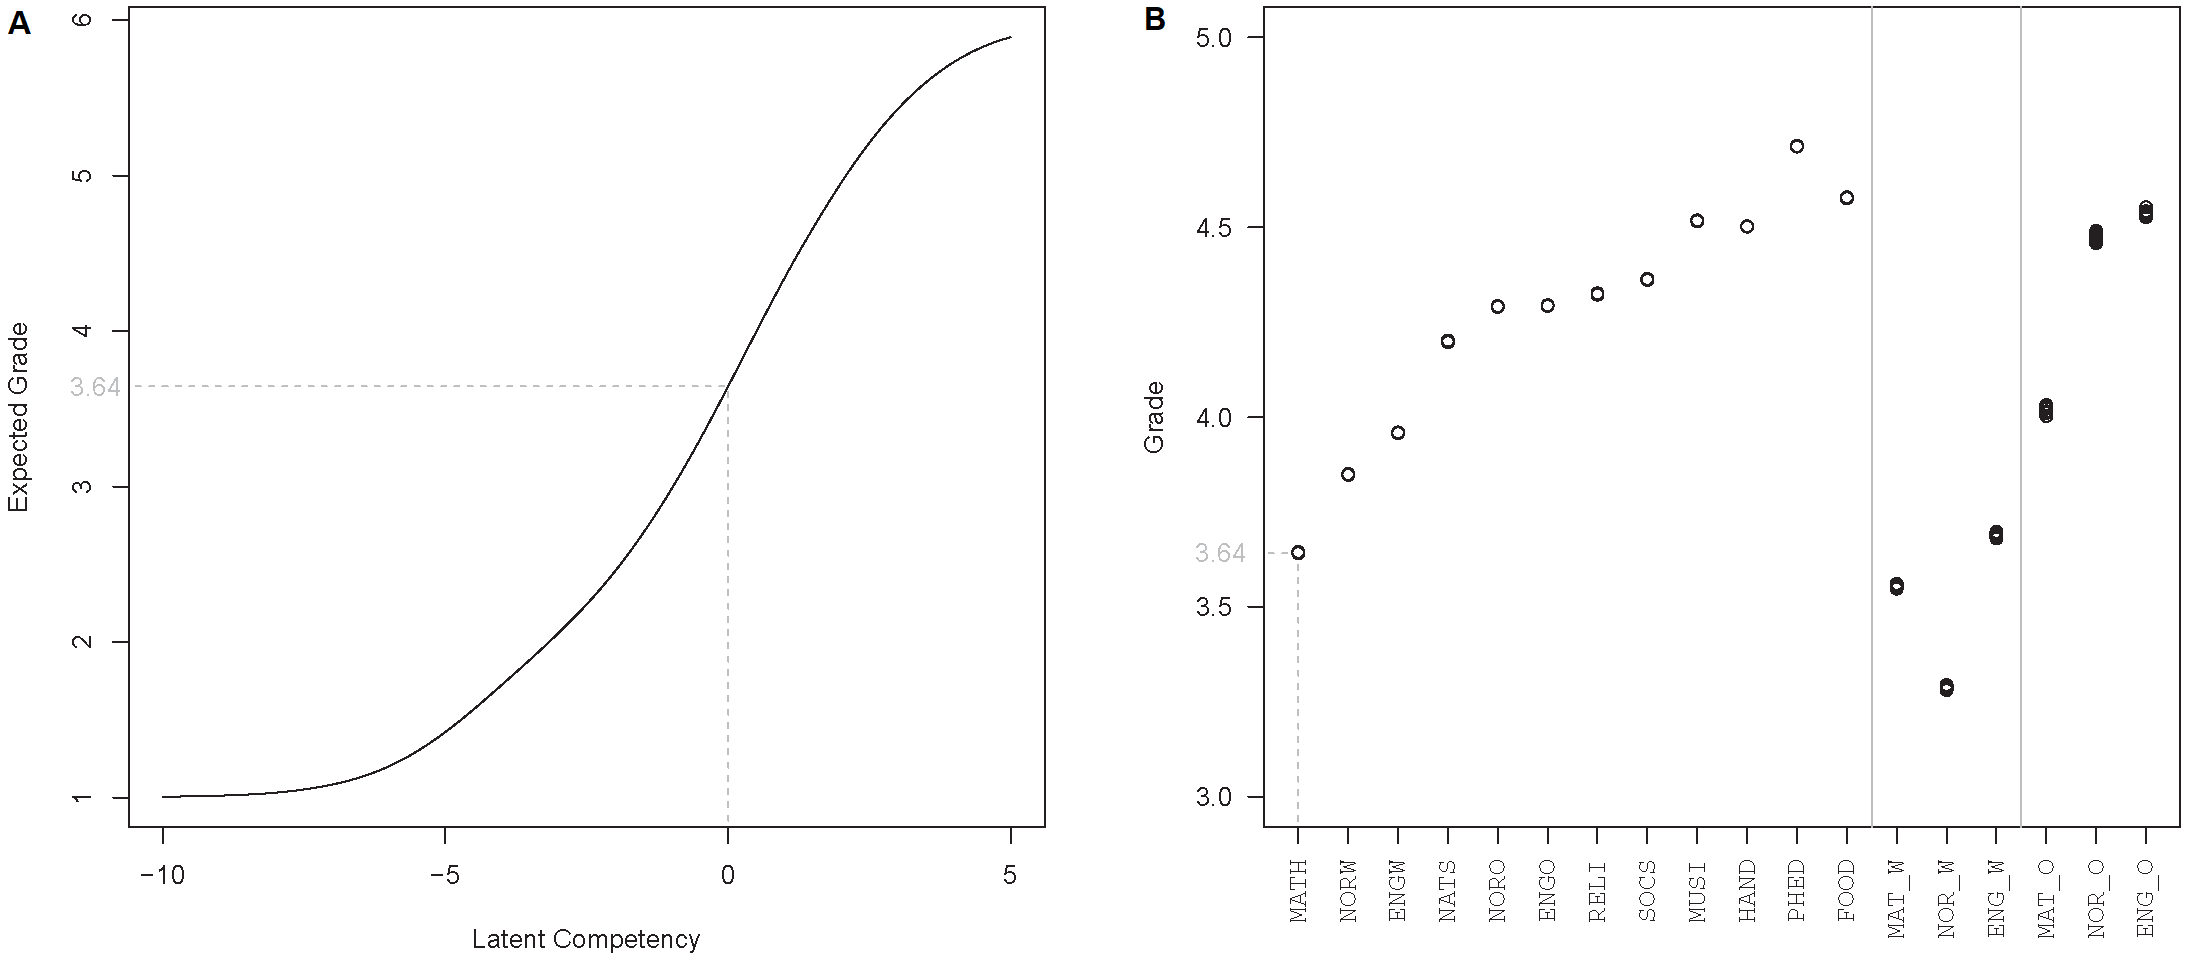
\includegraphics[width=1.5\textwidth]{./Figures/expected.png}
}{In Panel A, a median student evenly divides \textsc{math} candidates into 50\% below, and 50\% above him/her, whose $\theta$ is defined as zero. The expected grade of this median student 3.64 represents the \emph{overall difficulty} for \textsc{math}. Repeating this procedure for all 18 GPA subjects produces the scatter plot in Panel B. Subject with low expected grades such as \textsc{math} are more difficult while \textsc{phed} and \textsc{food} are easy subjects evidenced by the high expected grades from median students. Written- and oral-exams' overall difficulties are also shown. Results from ten imputed datasets were superimposed, leading to jitters in exam grades resultant from slightly larger imputation variations.}


\ttlfig{fig:grade_level}{Grade-level Difficulties}{
    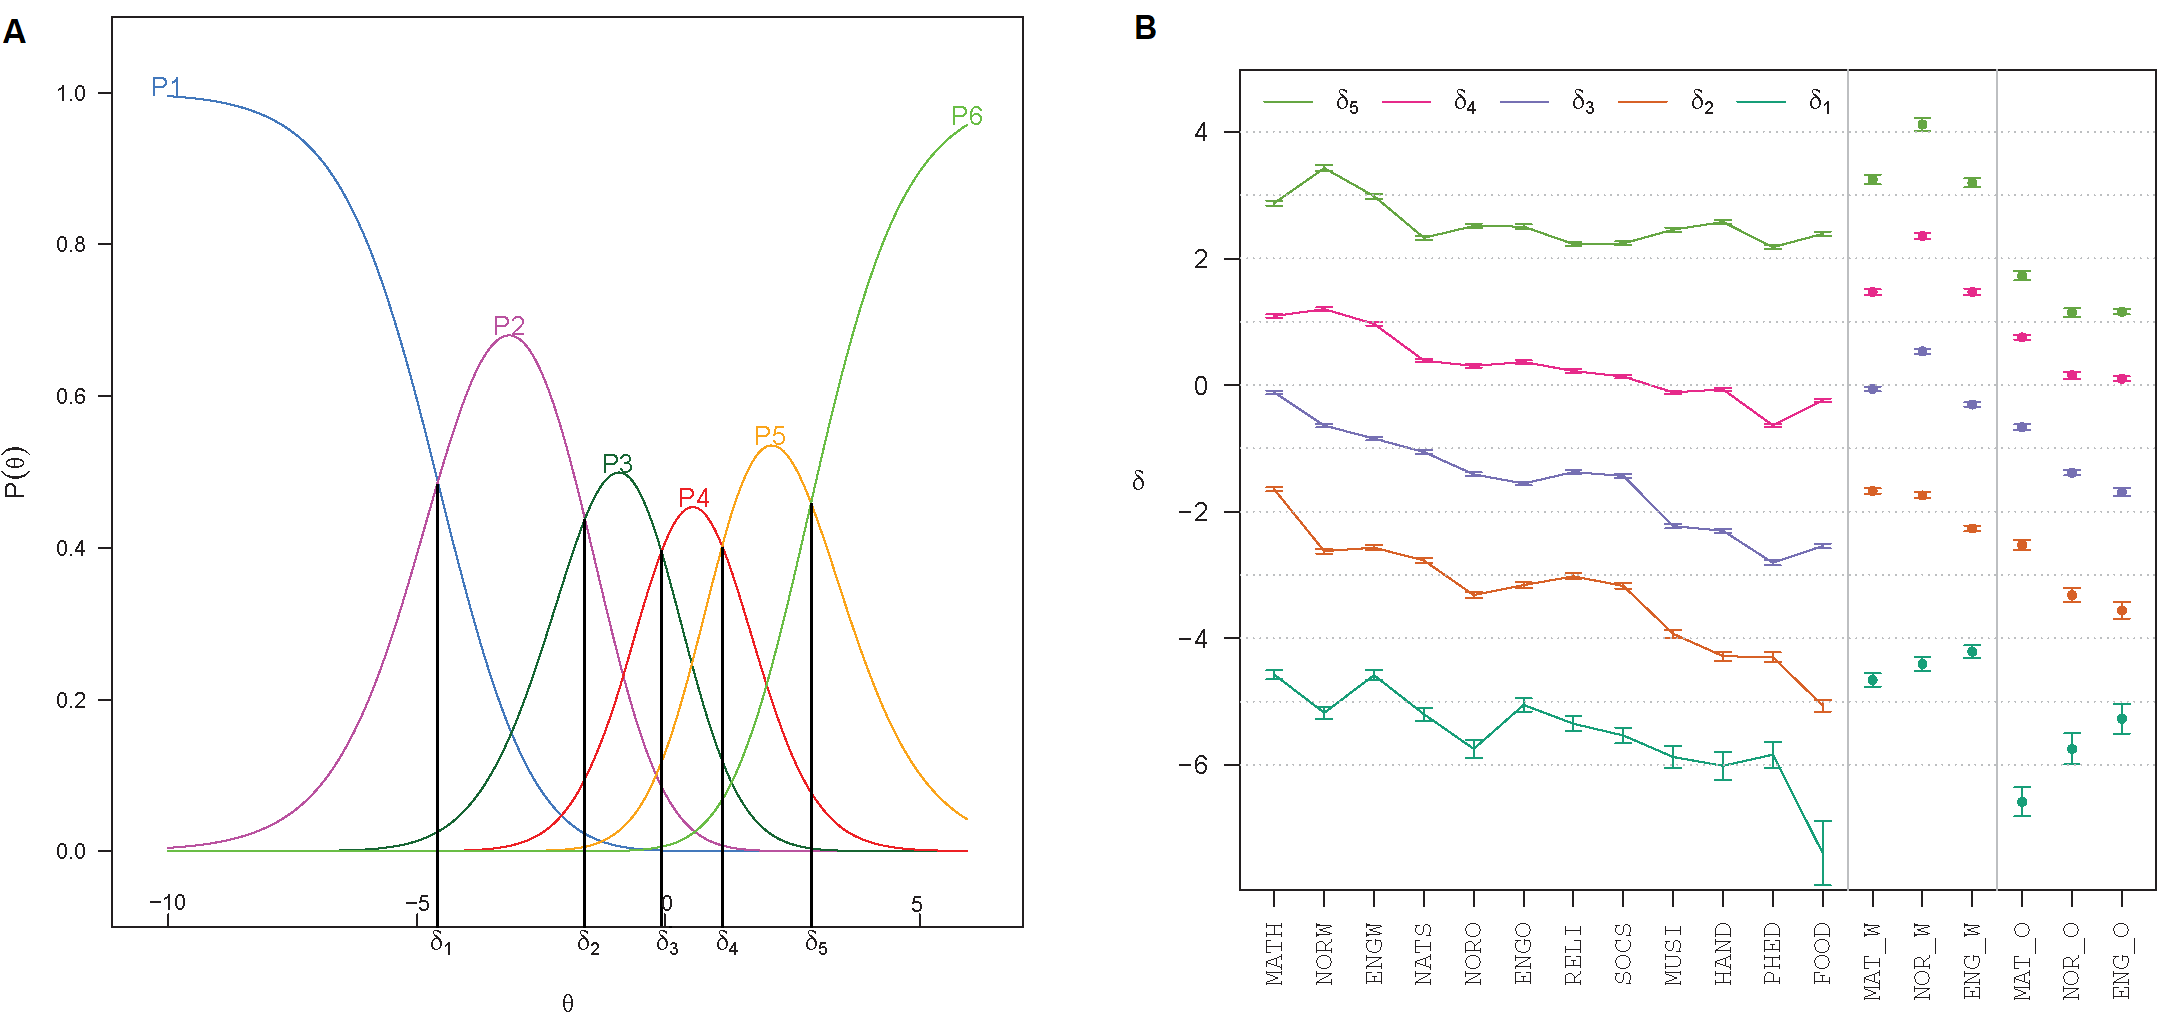
\includegraphics[width=1.5\textwidth]{./Figures/grade_level.png}
}{Panel A illustrates the category characteristic curve (\textsc{ccc}) for \textsc{math}. The vertical axis represents probabilities ranging from $0$ to $1$, and the horizontal axis represents students' latent competencies ranging from low ($\theta=-10$) to high ($\theta=5$). The \textsc{ccc} $P1$, for example, describes the association between competency levels and the likelihood students posessing this competency would receive Grade 1. The intersection between $P1$ and $P2$ marks a difficulty threshold $\delta_1$, above which Grade 2 is a more likely outcome. Six \textsc{ccc}s produce five thresholds $\delta_1, \dots, \delta_5$, which concisely summarise each subject's \emph{grade-level difficulties}. Repeating this procedure to all 18 \textsc{gpa} subjects produces Panel B. The 95\% confidence intervals are pooled over ten imputed datasets.}


\ttlfig{fig:fit}{Model Fit Measures}{
    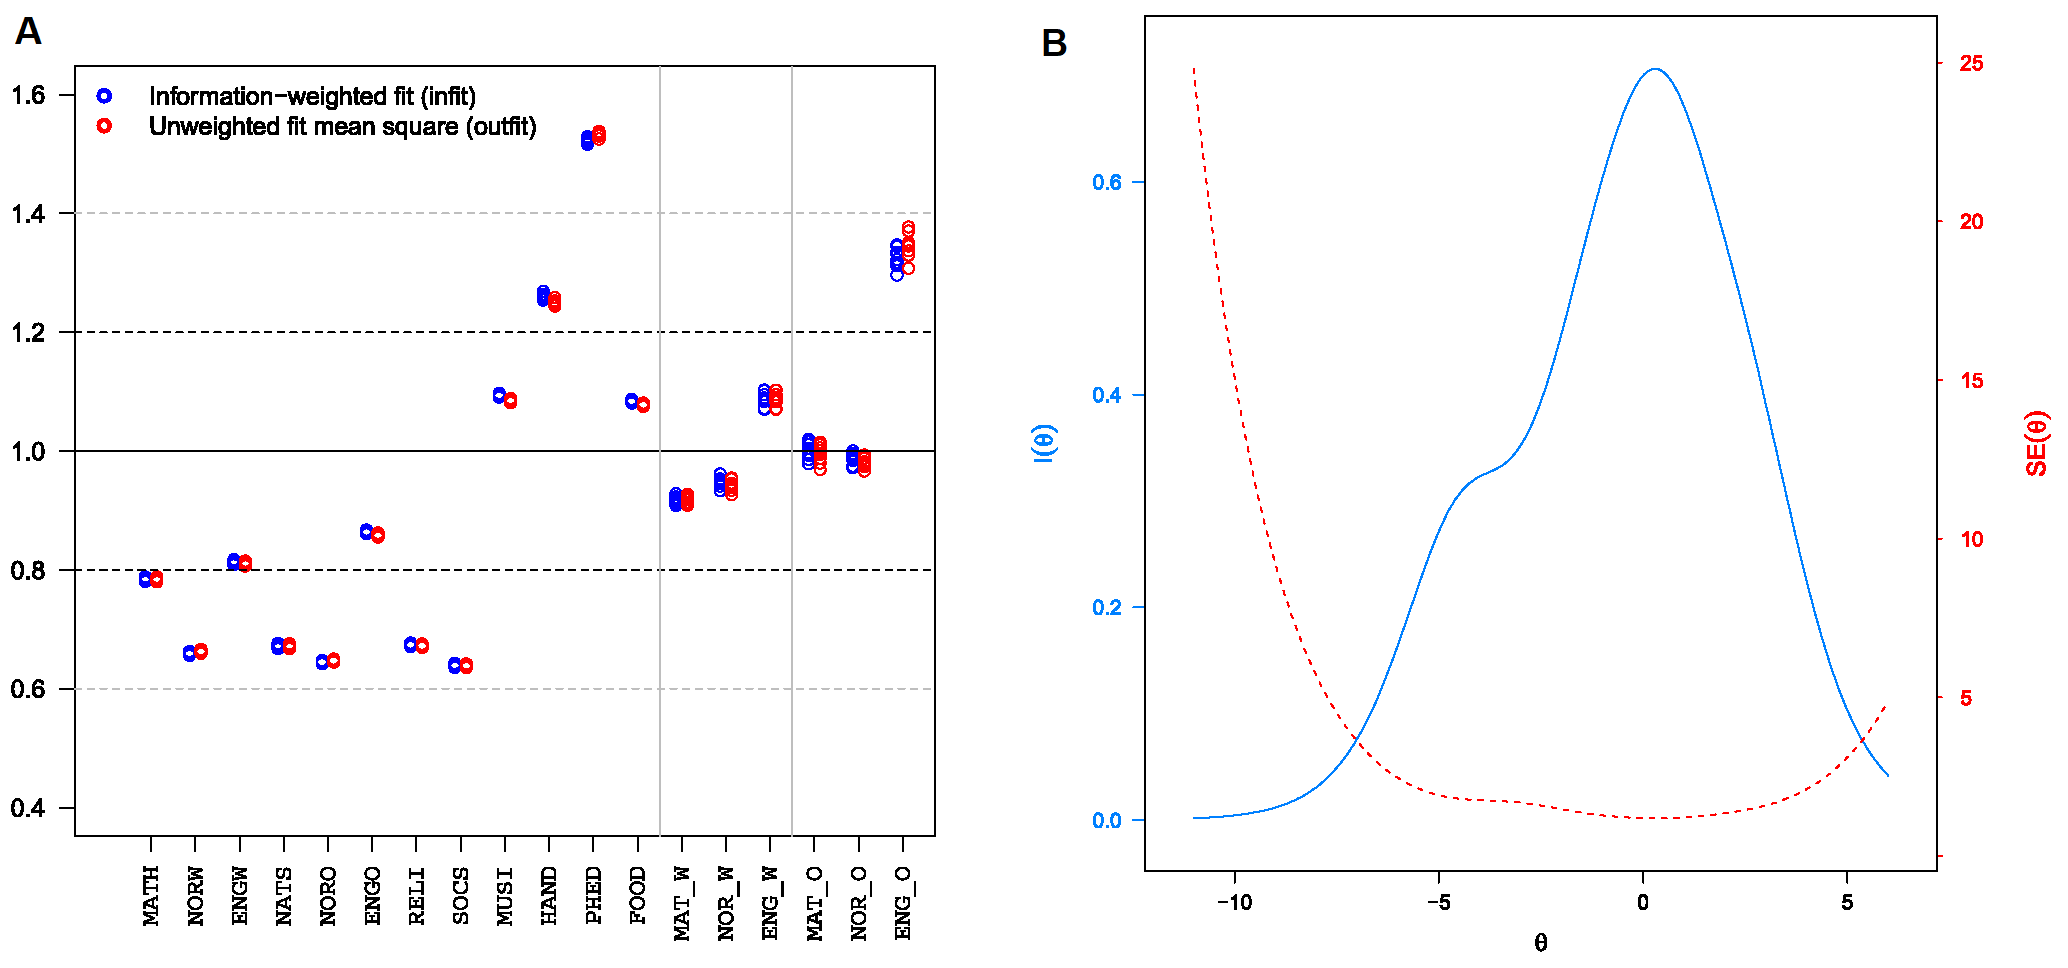
\includegraphics[width=1.5\textwidth]{./Figures/model_fit.png}
}{Panel A summarises model fit indices. A perfectly fit item in a Rasch model corresponds to infit and outfit statistics of $1$. Fit measure below $1$ indicate overfit where the item is more discriminating than the average item discrimination. Overfitting is usually not a problem comparing with underfitting. Empirical rules suggests close examination of items with infit and outfit statistics between $1.2$ and $1.5$ \parencite{wu:2016}. Panel B shows the information (blue, left scale) and standard error (red, right scale) curves of mathematics, suggesting good Rasch property over middle- to high-end of the competency scale.}


\ttpfig{fig:info}{Information and Standard Error Curves}{
    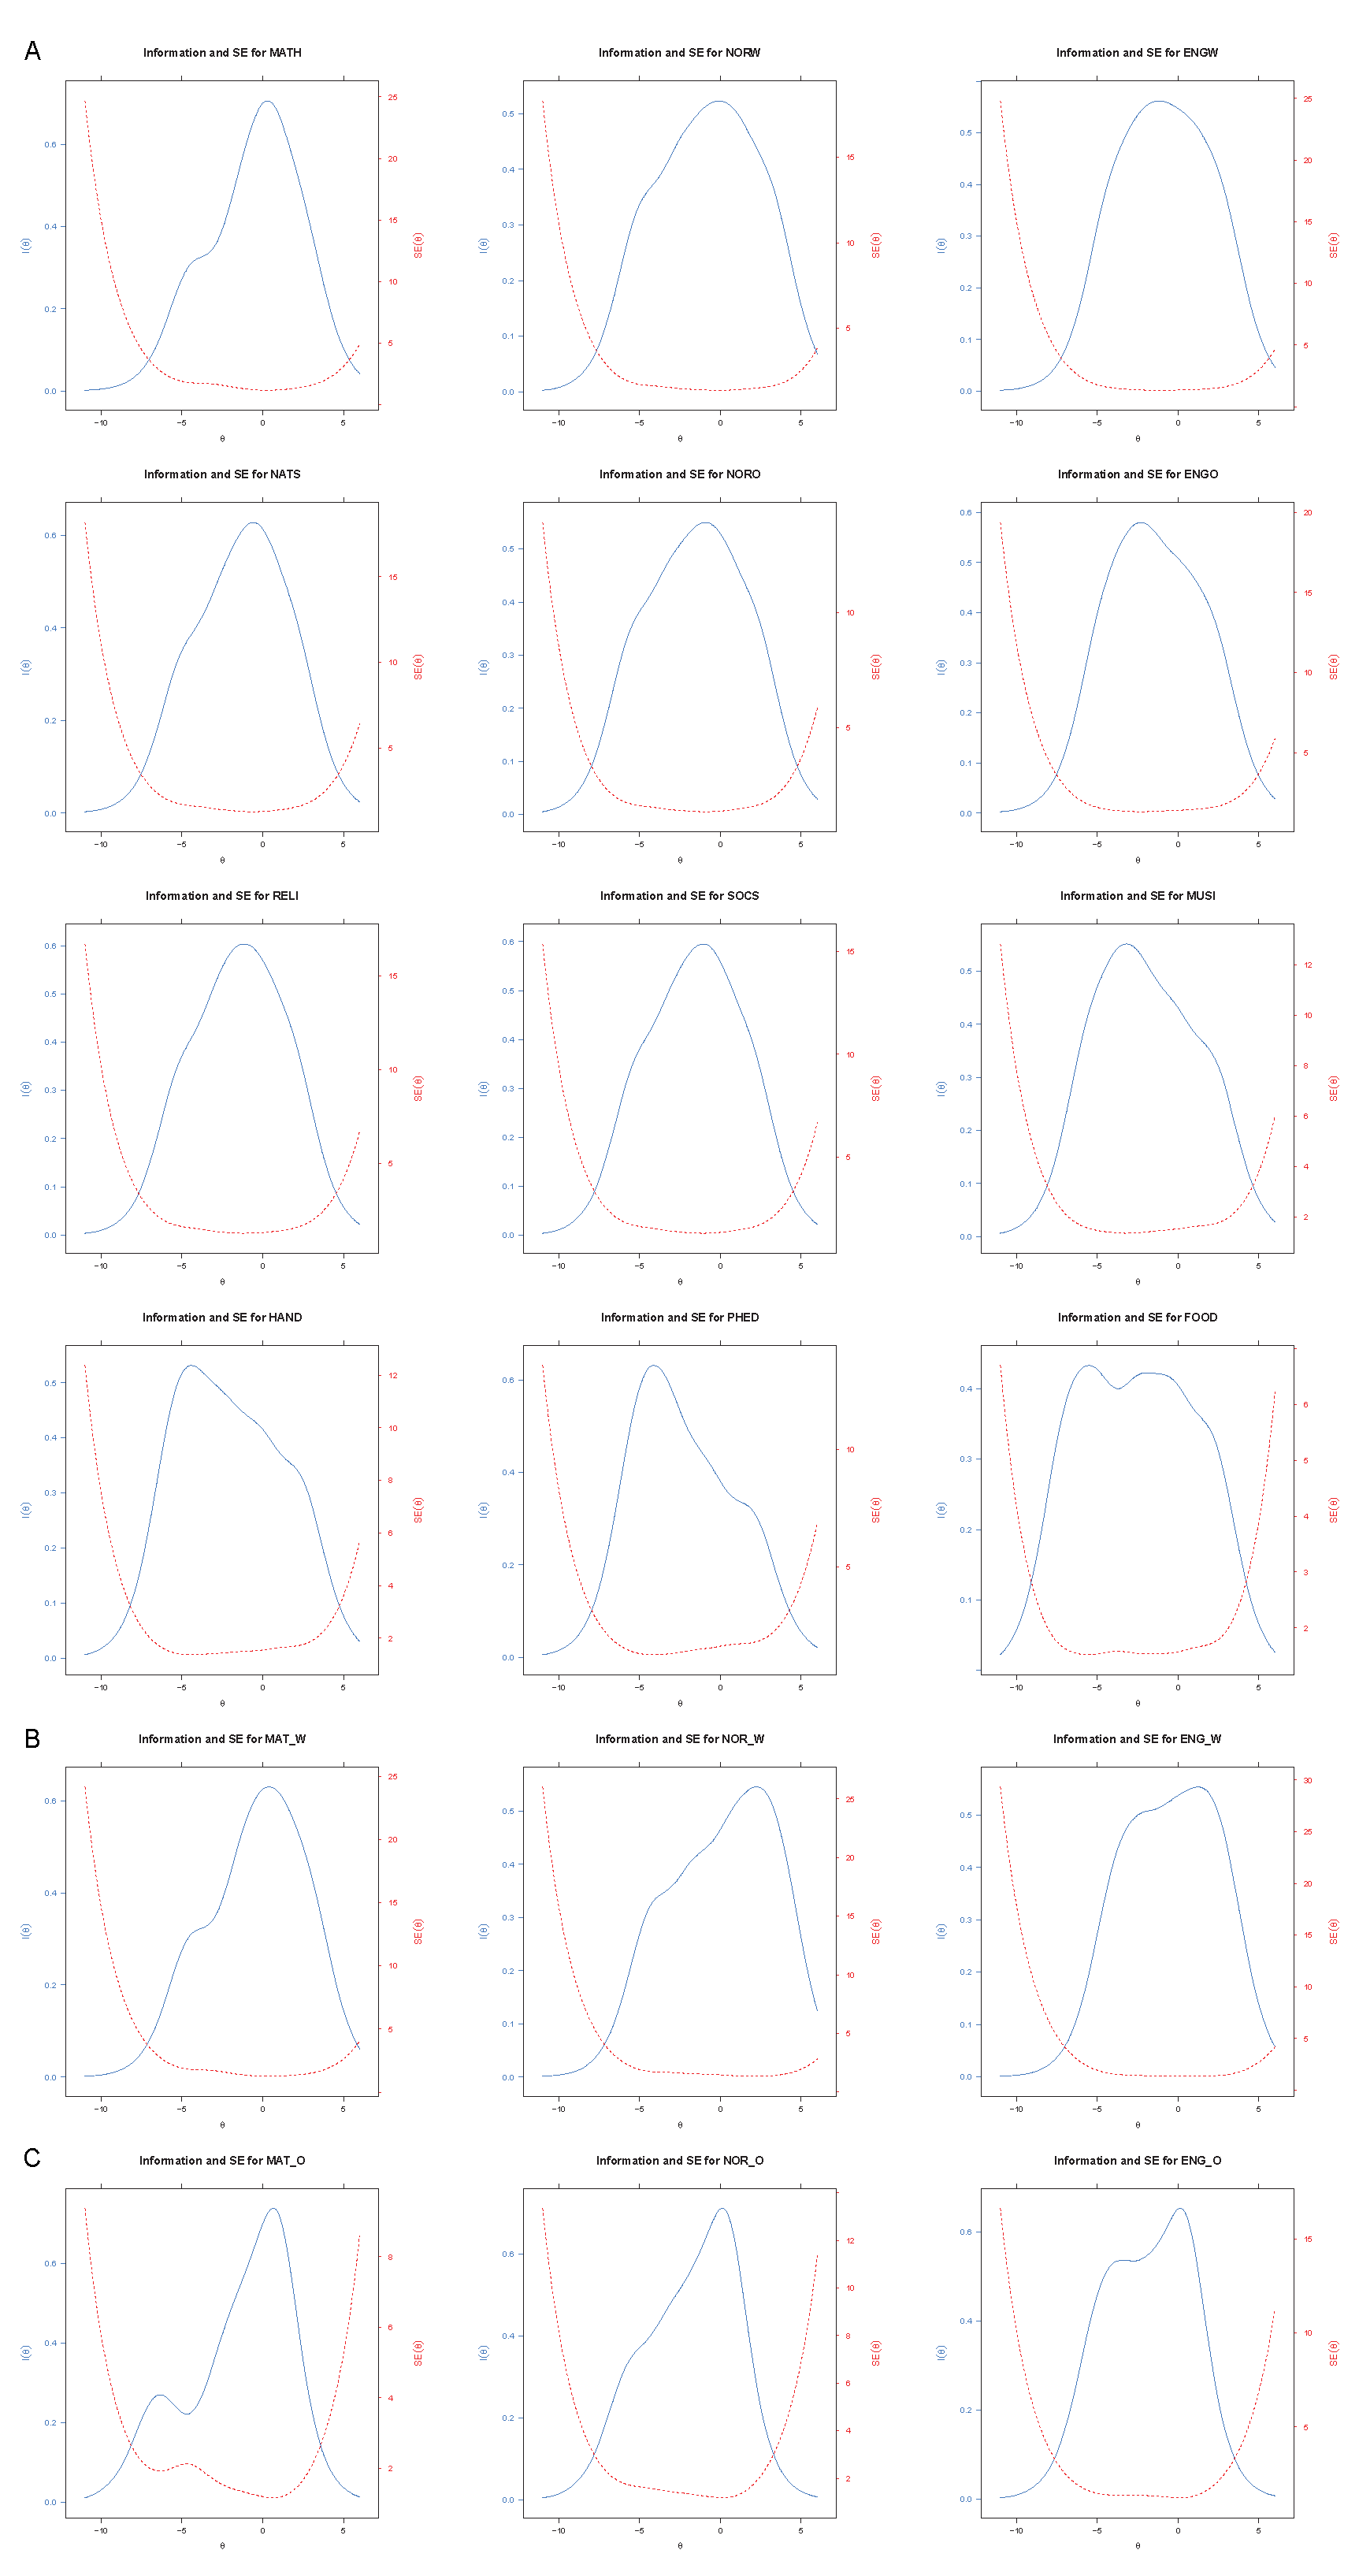
\includegraphics[width=\textwidth]{./Figures/info/info.png}
}{The information curves jointly suggest that all 18 \textsc{gpa} subjects under the Rasch model have high explanatory power over the mid-ranges of the competency scale where most students are located. The standard error curves show that the Rasch model is also more precise in the mid-competency range.}


%\section{Analysis Code, Additional Tables and Figures}\label{app}

% \subsection{Register Data Re-format}

% \begin{singlespacing}
%     \lstinputlisting[language=R,style=vscodeR,linerange={35-233}]{../Data/teacher.R}
% \end{singlespacing}

% \subsection{Retain Students with Valid GPA and Sufficient Teacher-assigned Grades}

% \begin{singlespacing}
%     \lstinputlisting[language=R,style=vscodeR,linerange={34-413}]{../Data/drop_no_gpa.R}
% \end{singlespacing}

% \subsection{Subject Difficulty Analysis using GPCM}

% \begin{singlespacing}
%     \lstinputlisting[language=R,style=vscodeR,linerange={35-101}]{../Data/irt.R}
% \end{singlespacing}

% \newpage

\subsection{IRT Analysis Output}

\ttptable{tab:par_pcm}{Partial Credit Model (PCM) Difficulty Parameters}{
    \begin{tabular}{clcrrrrrr}
        \toprule
        Subject Code & \multicolumn{1}{c}{Subject Name} & \multicolumn{1}{c}{$\E{x \mid \theta=0}$} & \multicolumn{1}{c}{$\tilde{\theta}$} & \multicolumn{1}{c}{$\delta_1$} & \multicolumn{1}{c}{$\delta_2$} & \multicolumn{1}{c}{$\delta_3$} & \multicolumn{1}{c}{$\delta_4$} & \multicolumn{1}{c}{$\delta_5$} \\
        \midrule
        \rowcolor[rgb]{ .851,  .851,  .851} NORW  & Written Norwegian & $3.85$ & $-0.71$ & $-5.953$ & $-3.062$ & $-0.805$ & $1.205$ & $3.605$ \\
        \rowcolor[rgb]{ .851,  .851,  .851} NORO  & Oral Norwegian & $4.29$ & $-1.54$ & $-6.313$ & $-3.724$ & $-1.633$ & $0.242$ & $2.622$ \\
        ENGW  & Written English & $3.96$ & $-0.87$ & $-5.189$ & $-2.967$ & $-1.017$ & $0.957$ & $3.138$ \\
        ENGO  & Oral English & $4.29$ & $-1.54$ & $-5.655$ & $-3.618$ & $-1.788$ & $0.310$ & $2.618$ \\
        \rowcolor[rgb]{ .851,  .851,  .851} MATH  & Mathematics & $3.64$ & $-0.22$ & $-4.934$ & $-1.856$ & $-0.213$ & $1.111$ & $3.028$ \\
        \rowcolor[rgb]{ .851,  .851,  .851} NATS  & Natural Sciences & $4.20$ & $-1.18$ & $-5.724$ & $-3.085$ & $-1.226$ & $0.345$ & $2.433$ \\
        SOCS  & Social Sciences & $4.36$ & $-1.55$ & $-6.065$ & $-3.519$ & $-1.638$ & $0.071$ & $2.333$ \\
        RELI  & Religion and Ethics & $4.33$ & $-1.46$ & $-5.822$ & $-3.374$ & $-1.583$ & $0.152$ & $2.325$ \\
        \rowcolor[rgb]{ .851,  .851,  .851} MUSI & Music & $4.51$ & $-2.23$ & $-6.305$ & $-4.288$ & $-2.471$ & $-0.198$ & $2.557$ \\
        HAND  & Arts and Handcraft & $4.50$ & $-2.74$ & $-6.447$ & $-4.599$ & $-2.522$ & $-0.143$ & $2.687$ \\
        \rowcolor[rgb]{ .851,  .851,  .851} FOOD  & Food and Health & $4.57$ & $-2.66$ & $-7.768$ & $-5.455$ & $-2.791$ & $-0.336$ & $2.485$ \\
        PHED  & Physical Education & $4.70$ & $-2.66$ & $-6.221$ & $-4.607$ & $-3.035$ & $-0.730$ & $2.265$ \\
        \bottomrule
        \end{tabular}%
}{A partial credit model (PCM) computes the expected grades of an average candidate ($\E{x \mid \theta=0}$), the overall subject difficulties ($\tilde{\theta}$), and difficulty thresholds ($b_1$ to $b_5$) for each adjacent grades. A lower expected grade corresponds to a harder subject while higher $\tilde{\theta}$ signals a more difficult subject. A higher $b$ indicates that it takes higher capability, hence more difficult, to transition onto the next grade level. All estimates are significant at $.001$ level.}





\newpage


\end{document}
